\section{Data resources and use scenarios}
\label{sect:motivation}

FMA - taxonomy, connectivity data

Genes ontology

CellML

3D models


We arrange data in a hierarchical way starting from the large-scale views showing external and internal surfaces and organs
arranged to resemble the longitudinal section through the middle of the human body as the top-level taxonomy.
Figure~\ref{fig:application} shows the idealized radially symmetric body plan, apportioned over cylindrical regions.
This homunculus has a central longitudinal axis of rotation located in the idealized gut lumen which runs in the cephalocaudal direction.
Each of the organs in the plan is composed of multiple tissues and sub-organs, the structural information about them is obtained from the Foundational Model of Anatomy (FMA) ontology\footnote{Foundational Model of Anatomy -
\textsf{http://sig.biostr.washington.edu/projects/fm/}}. As the visualization of the full ontology may obscure the details a user is interested to see, it is essential for the visualization tool to support data filtering across multiple levels and contextual zooming into selected areas. The user should be able to create a custom view with the internal structure of the selected body parts placed in a way that simplifies the analysis of these data.

\begin{figure*}
\centering
  \subfigure[Schematic body plan]{
    \label{fig:anatomy}
    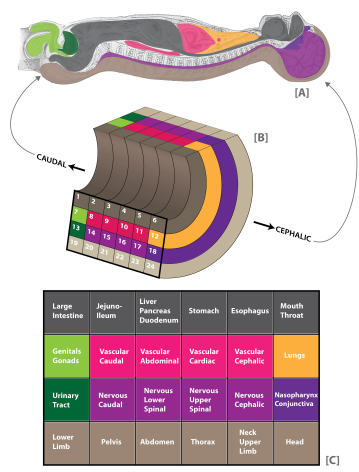
\includegraphics[width=4.3cm]{images/application.png}
  }
  \subfigure[Visualizing medical ontologies using treemaps]{
  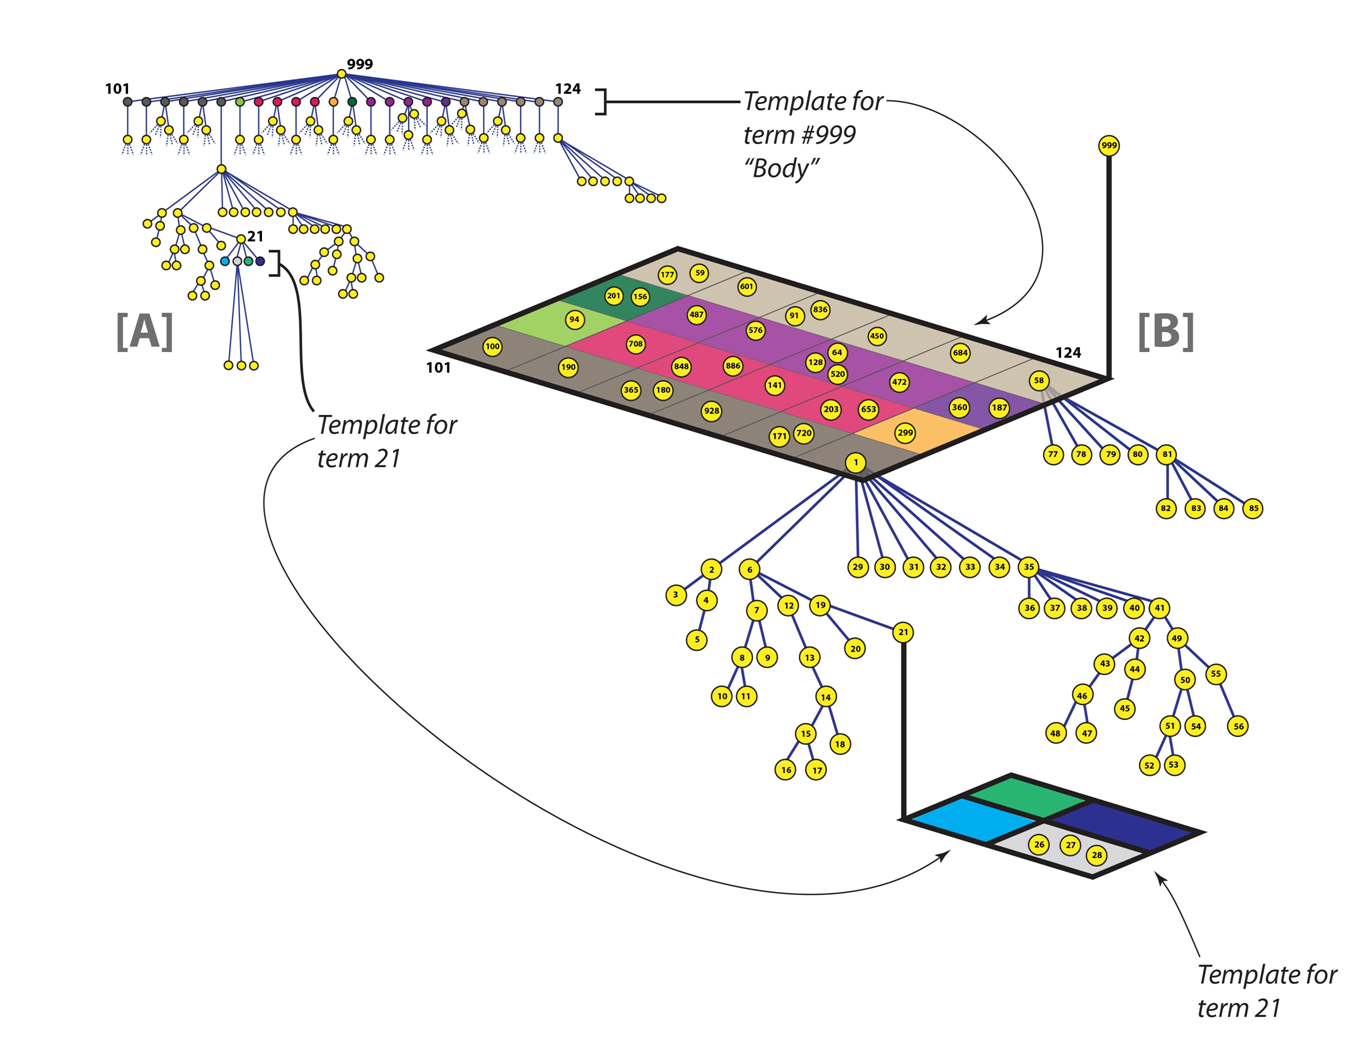
\includegraphics[width=7.3cm]{images/application1.png}
  }
  \caption{Longitudinal section through the middle of the male human body}
  \label{fig:application}
\end{figure*}

